\RequirePackage{atbegshi}
\documentclass{beamer}

\usepackage{graphicx,epstopdf,subfigure,booktabs,natbib,fancyvrb}
\usepackage{tikz}
\usetikzlibrary{arrows,shapes,positioning,trees,mindmap,backgrounds}

%\usetheme[compress,subsection=F]{Singapore}
%\useoutertheme[subsection=false]{miniframes}
\usetheme[hideallsubsections]{Hannover}
%\usecolortheme{dove}
\usecolortheme{seagull}
\useinnertheme{default}

\bibliographystyle{plainnat}
\bibpunct{[}{]}{;}{a}{}{,}
\usefonttheme{serif}
\usepackage{mathpazo}

\definecolor[named]{Yellow}{cmyk}{.01,.11,.74,0}
\definecolor[named]{Red}{cmyk}{0,.48,.62,0}
\definecolor[named]{Green}{cmyk}{.31,0,.69,0}
\definecolor[named]{Teal}{cmyk}{.39,.05,.18,0}
\definecolor[named]{Purple}{cmyk}{.16,.31,0,0}
\definecolor[named]{Gray}{cmyk}{0,0,0,.29}

\tikzset{em/.style ={
        fill=Yellow,
        draw=black,
		thick, 
    },
    brackish/.style={
        fill=Red, 
        draw=black,
		thick,
    },
    ox/.style={
        fill=Green,
        draw=black,
		thick, 
    },
    contact/.style={
        fill=Purple,
        draw=black,
		thick, 
    },
    tm/.style={
        fill=Teal, 
        draw=black,
		thick,
    },    
    txt/.style ={
		text width=5em,
		text centered
    },
    pump/.style ={
        draw,
        thick,
        double distance=1pt,
        -latex'
    },
    gravity/.style ={
        draw,
        thick,
        -stealth,
    },
    double/.style ={
        draw,
        thick,
        stealth-stealth,
    },
    phantom/.style = {
    		none,
    	    inner sep=-10,
		outer sep=1pt,
		node distance=1mm
	}}

\title[Past, Present and Future Work]{Reclamation Review of Stochastic Streamflow Simulation at Interannual and Interdecadal Time Scales and Implications to Water Resources Management}
\subtitle{Past, Present and Future Work}
\author[\it Cameron Bracken]{{\it Cameron Bracken}\small\\M.S. Student\\CADSWES, CU Boulder\\October 29th, 2010}
\date{{\it Principle Investigators}:\small\\Edie Zagona, CADSWES\\Balaji Rajagopalan, CU}

\begin{document}

%%%%%%%%%%%%%%%%%%%%%%%%%%%%%%%%%%%%%%%%%%%%%%%%%%%%%%
%%%%%%%%%%%%%%%%%%%%%%%%%%%%%%%%%%%%%%%%%%%%%%%%%%%%%%
\begin{frame}
\titlepage
\end{frame}

%%%%%%%%%%%%%%%%%%%%%%%%%%%%%%%%%%%%%%%%%%%%%%%%%%%%%%
%%%%%%%%%%%%%%%%%%%%%%%%%%%%%%%%%%%%%%%%%%%%%%%%%%%%%%
\section{24 Month Study}
\begin{frame}{24 Month Study}
\begin{itemize}
	\item BOR's Monthly midterm operational forecast model for the CRB
	\item Inputs: 
		\begin{itemize}
			\item Unregulated inflows (RFC $\sim$1 year, climatology after)
			\item Releases manually input by individual dam operators
		\end{itemize}
	\item Outputs: 
	\begin{itemize}
		\item Power, Evap, Elevation, Storage, etc. 
	\end{itemize}
\end{itemize}
\end{frame}

%%%%%%%%%%%%%%%%%%%%%%%%%%%%%%%%%%%%%%%%%%%%%%%%%%%%%%
%%%%%%%%%%%%%%%%%%%%%%%%%%%%%%%%%%%%%%%%%%%%%%%%%%%%%%
\section{Probabilistic Midterm Model}
\begin{frame}{Probabilistic Midterm Model}
\begin{itemize}
\item Midterm operational forecast model for the CRB
\item Probablistic version 24 month study
\item New features
\end{itemize}
\pause

\begin{center}
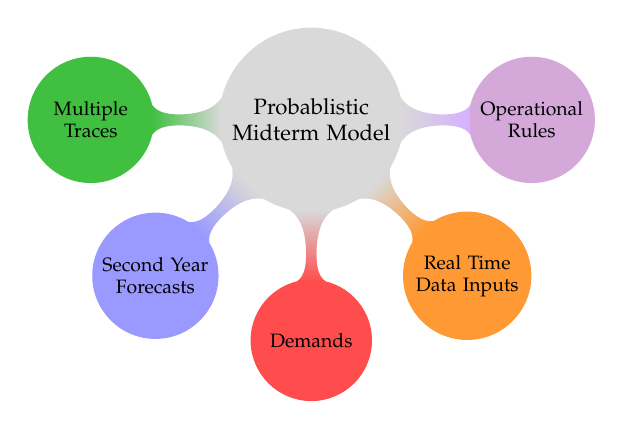
\begin{tikzpicture} [small mindmap,level 1 concept/.append style={sibling angle=45}]
	\path[mindmap,concept color=gray!30] 
		node[concept] {Probablistic Midterm Model} [counterclockwise from=180] 
			child[concept color=green!50!gray] { node[concept] {Multiple Traces} }
			child[concept color=blue!40] { node[concept] {Second Year Forecasts} 
				% [clockwise from=-30] 
				%	child[concept color=purple!40] { node[concept] {Operational Mode} } 
				%	child[concept color=purple!40] { node[concept] {Analysis Mode} }
			} 
			child[concept color=red!70] { node[concept] {Demands} }
			child[concept color=orange!80] { node[concept] {Real Time Data Inputs} }
			child[concept color=Purple] { node[concept] {Operational Rules} 
		}; 
\end{tikzpicture} 
\end{center}

\end{frame}

%%%%%%%%%%%%%%%%%%%%%%%%%%%%%%%%%%%%%%%%%%%%%%%%%%%%%%
%%%%%%%%%%%%%%%%%%%%%%%%%%%%%%%%%%%%%%%%%%%%%%%%%%%%%%
\section{Modeling Operations}
\begin{frame}{Modeling Operations}

\begin{itemize}
	\item Actual operations are a combination of many factors:
	
	\begin{itemize}
		\item Law (EIS's)
		\item Guidelines (Power Generation)
		\item Daily Targets
		\item Monthly or Seasonal Targets
		\item Peak Flows
		\item Base Flow
		\item Extreme Events (Dam Safety Operations)
		\item MANY More...
	\end{itemize}
\end{itemize}
\end{frame}

%%%%%%%%%%%%%%%%%%%%%%%%%%%%%%%%%%%%%%%%%%%%%%%%%%%%%%
%%%%%%%%%%%%%%%%%%%%%%%%%%%%%%%%%%%%%%%%%%%%%%%%%%%%%%
\section{Example}
\begin{frame}{Example}
\framesubtitle{Operator Notes}
\begin{itemize}
\item Baseflows: steady release mid August to mid April (usually 1000-1200 cfs)
	\begin{itemize}
		\item Flows are steady to protect fish (spawning, etc.) and to prevent flooding due to ice jamming
		\item Set flow to put reservoir at March/April 6468ft target
	\end{itemize}
\end{itemize}
\end{frame}

%%%%%%%%%%%%%%%%%%%%%%%%%%%%%%%%%%%%%%%%%%%%%%%%%%%%%%
%%%%%%%%%%%%%%%%%%%%%%%%%%%%%%%%%%%%%%%%%%%%%%%%%%%%%%
\begin{frame}{Example}
\framesubtitle{Rule Outline}

\textbf{Set December-March Baseflow}

\textit{Execution Constraint}: Month is December

\textit{Description}: Set December-March outflow to steady value that will meet ``April 1 Target Elevation''

\begin{itemize}
	\item Compute change in volume given ``April 1 Target Elevation'' and current elevation
	\item Add volume gain from forecasts December-March (4 months)
	\item Compute max steady flow over December-March (4 months)
\end{itemize}
\end{frame}

%%%%%%%%%%%%%%%%%%%%%%%%%%%%%%%%%%%%%%%%%%%%%%%%%%%%%%
%%%%%%%%%%%%%%%%%%%%%%%%%%%%%%%%%%%%%%%%%%%%%%%%%%%%%%
\begin{frame}
\frametitle{Example}
\framesubtitle{RPL Rule}

\includegraphics[width=\textwidth]{figs/rpl.pdf}

%\begin{verbatim}
%Fontenelle.Outflow[] = 
%    ( ElevationToStorage( %"Fontenelle", Fontenelle.Pool Elevation[@"t"] ) - 
%    ElevationToStorage(%"Fontenelle", FontenelleData.April1Target[] ) + 
%    SumFlowsToVolume( Fontenelle.Inflow, @"t",@"t + 3" ) ) / 4.00000000 "month"
%\end{verbatim}

%Execution Constraint 

%\begin{verbatim}
%GetMonthAsString( @"t" ) IN { "December" }
%\end{verbatim}
 
 \end{frame}

%%%%%%%%%%%%%%%%%%%%%%%%%%%%%%%%%%%%%%%%%%%%%%%%%%%%%%
%%%%%%%%%%%%%%%%%%%%%%%%%%%%%%%%%%%%%%%%%%%%%%%%%%%%%%
\section{Rules Development}
\begin{frame}{Rules Development: From Management to Model}
For Each Reservoir:

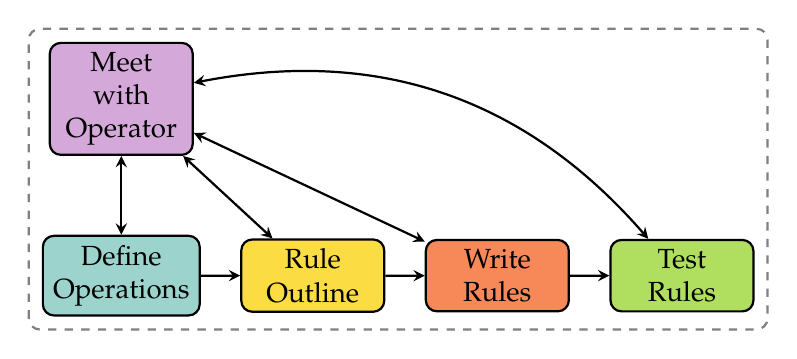
\begin{tikzpicture}
    [
    node distance=10mm and 5mm,
    scale=.6,
    text width=4.5em,
    text centered,
    rectangle,
    rounded corners,
    show background rectangle,
    background rectangle/.style={
		draw=gray,
		thick,
		dashed,
		rounded corners
	}
    ]

    \node(meet) [contact] {Meet with Operator};
    \pause
    
    \node(define) [tm,below=of meet,text width=5em] {Define Operations};
    \path[double] (meet) -- (define);
    \pause 
    
    \node(outline) [em,right=of define] {Rule Outline};
    \path[gravity] (define) -- (outline);
    \pause
    
    \path[double] (meet) -- (outline);
    \pause
    
    \node(rules) [brackish,right=of outline] {Write Rules};
    \path[gravity] (outline) -- (rules);
    \pause
    
    \path[double] (meet) -- (rules);
    \pause
    
    \node(test) [ox,right=of rules] {Test Rules};
    \path[gravity] (rules) -- (test);
	\pause
	
	\path[double] (meet) edge[bend left] (test);
    \pause
	
\end{tikzpicture}
\end{frame}

%%%%%%%%%%%%%%%%%%%%%%%%%%%%%%%%%%%%%%%%%%%%%%%%%%%%%%
%%%%%%%%%%%%%%%%%%%%%%%%%%%%%%%%%%%%%%%%%%%%%%%%%%%%%%
\section{Implications}
\begin{frame}{Implications}
\begin{itemize}
\item Self-documenting process
\item Testing gets harder as more reservoirs are added
\item Many operations don't translate perfectly to a monthly model

\item Rules must be very robust for different model start dates and hydrologic conditions
\begin{itemize}
\item Lots of checking which month it is!
\end{itemize}
\item ...3,2,1 rule ordering is crucial
\end{itemize}
\end{frame}

%%%%%%%%%%%%%%%%%%%%%%%%%%%%%%%%%%%%%%%%%%%%%%%%%%%%%%
%%%%%%%%%%%%%%%%%%%%%%%%%%%%%%%%%%%%%%%%%%%%%%%%%%%%%%
\section{Work so far}
\begin{frame}{Work So Far}
\begin{itemize}
\item Rules written and tested for Fontenelle, Flaming Gorge, Navajo
\item Lake Powell rules written but not thoroughly tested.
\item Model and rules are assembled
\item Aspinall need to be written
\item Tons of testing
\end{itemize}
\end{frame}

%%%%%%%%%%%%%%%%%%%%%%%%%%%%%%%%%%%%%%%%%%%%%%%%%%%%%%
%%%%%%%%%%%%%%%%%%%%%%%%%%%%%%%%%%%%%%%%%%%%%%%%%%%%%%
\section{Interannual Water Supply Forecasting}

%%%%%%%%%%%%%%%%%%%%%%%%%%%%%%%%%%%%%%%%%%%%%%%%%%%%%%
%%%%%%%%%%%%%%%%%%%%%%%%%%%%%%%%%%%%%%%%%%%%%%%%%%%%%%
\section{Past Work}
\subsection{REU Project}
\begin{frame}{Past Work - REU Project}
\pause
The goal of the project was to: 
\begin{itemize}
  \item Develop a \alert{seasonal streamflow forecast framework}
\begin{itemize}

\item Handle many spatial locations 
\item Preserve spatial and temporal dependencies
\item Incorporate large scale climate predictors
\item Use modern nonparametric methods
\item Generate multi-model ensembles
\end{itemize}
\end{itemize}


\end{frame}

%%%%%%%%%%%%%%%%%%%%%%%%%%%%%%%%%%%%%%%%%%%%%%%%%%%%%%
%%%%%%%%%%%%%%%%%%%%%%%%%%%%%%%%%%%%%%%%%%%%%%%%%%%%%%
\subsection{Seasonal Flow Forecast Framework}
\begin{frame}{Past Work}
%\beginpgfgraphicnamed{figs/framework}
%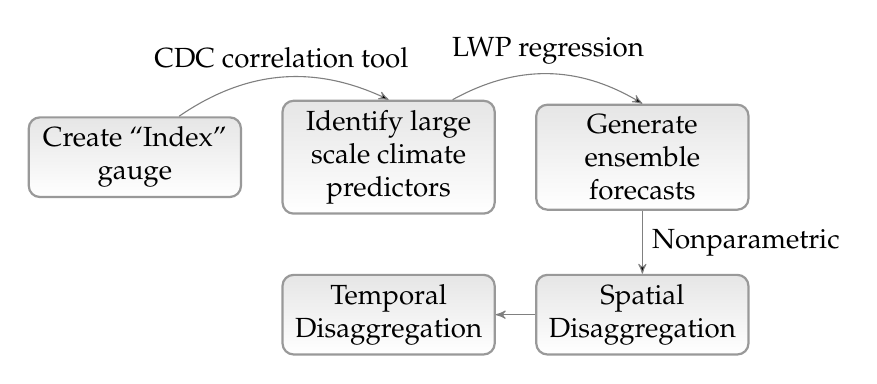
\begin{tikzpicture}
    [
    node distance=8mm and 5mm,
    block/.style ={
        rectangle, 
        draw=gray!80, 
        thick, 
        top color=gray!20, 
        bottom color=white,
        text badly centered, 
        text width=7em,
        rounded corners
    },
    a/.style={
        -stealth',
        draw=gray
    }
    ]
    \node (index)[block] {Create ``Index'' gauge};
    \node (predictors)[block,right=of index] {Identify large scale climate predictors};
    \node (ensemble)[block,right=of predictors] {Generate ensemble forecasts};
    \node (spatial)[block,below=of ensemble] {Spatial Disaggregation};
    \node (temporal)[block,left=of spatial] {Temporal Disaggregation};
      
    \draw[a] (index) edge [bend left] node [above] {CDC correlation tool} (predictors.90);
    \draw[a] (predictors) edge [bend left] node [above] {LWP regression} (ensemble.90);
    \draw[a] (ensemble) edge node [right] {Nonparametric} (spatial);
    \draw[a] (spatial) -- (temporal);
    
\end{tikzpicture}

%\endpgfgraphicnamed
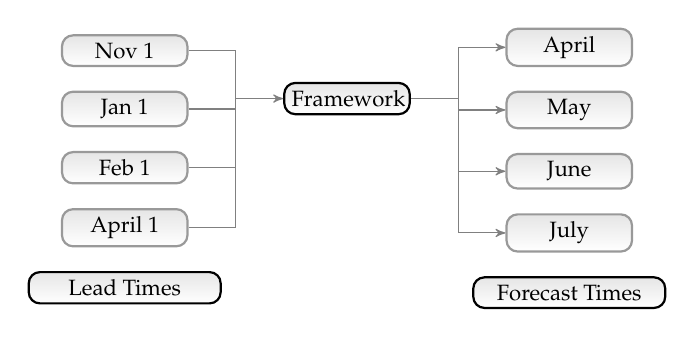
\begin{tikzpicture}
    [
    node distance=3mm and 5mm,
    block/.style ={
        rectangle, 
        draw=gray!80, 
        thick, 
        top color=gray!20, 
        bottom color=white,
        text badly centered, 
        text width=5em,
        rounded corners
    },
    phantom/.style={
        inner sep=0,
        outer sep=-.7pt,
    },
    a/.style={
        -stealth',
        draw=gray
    },
    l/.style={
        draw=gray
    }
    ]
    \footnotesize
    \node (lead1)[block] {Nov 1};
    \node (lead2)[block,below=of lead1] {Jan 1};
    \node (lead3)[block,below=of lead2] {Feb 1};
    \node (lead4)[block,below=of lead3] {April 1};
    \node (leaddes)[block,draw=black,text width=8em,below=of lead4] {Lead Times};
    
    \node (p1)[below right=of lead1]{};
    
    \node (f)[block,right=of p1,draw=black] {Framework};
    
    \node (p2)[right=of f]{};
    
    \node (fc1)[block,above right=of p2] {April};
    \node (fc2)[block,below=of fc1] {May};
    \node (fc3)[block,below=of fc2] {June};
    \node (fc4)[block,below=of fc3] {July};
    \node (fcdes)[block,draw=black,text width=8em,below=of fc4] {Forecast Times};
      
    \draw[l] (lead1) -| (p1.center);
    \draw[l] (lead2) -| (p1.center);
    \draw[l] (lead3) -| (p1.center);
    \draw[l] (lead4) -| (p1.center);
    
    \draw[a] (p1.center) -- (f);
    
    \draw[a] (p2.center) |- (fc1);
    \draw[a] (p2.center) |- (fc2);
    \draw[a] (p2.center) |- (fc3);
    \draw[a] (p2.center) |- (fc4);
    
    \draw[l] (p2.center) -- (f);
    
\end{tikzpicture}

\begin{figure}[htbp]
   \centering
   \includegraphics[width=.9\textwidth]{figs/framework.pdf} 
   %\caption{Seasonal flows at Lees Ferry}
\end{figure}

\end{frame}

\section{Current Work}
\subsection{Application to All Upper Basin Natural Flow Nodes}
\begin{frame}{Application to All Upper Basin Natural Flow Nodes}

\begin{columns}
\begin{column}{.5\textwidth}
\only<1>{
\begin{itemize}
\item Expand to all 20 natural flow nodes in the upper basin
\item Forecast in Total flow space but convert to intervening
\item Update predictors and natural flow data to most recent available (2007)
\end{itemize}
}
\only<2>{
\includegraphics[width=\textwidth]{figs/intervening-to-total-schematic.pdf}
}
\end{column}
\begin{column}{.5\textwidth}
\includegraphics[width=\textwidth]{figs/natural-flow-nodes.pdf}
\end{column}
\end{columns}
\end{frame}
\subsection{Preliminary Results}
\begin{frame}{Preliminary Results}
\tiny
\begin{table}[!ht]
\begin{center}
\caption{Jan 1 RPSS after disaggregation}
\begin{tabular}{rrrrr}
  \toprule  & April & May & June & July \\ 
  \midrule Colorado River At Glenwood Springs, CO & -0.09 & 0.03 & 0.03 & 0.04 \\ 
  Colorado River Near Cameo, CO & 0.15 & 0.06 & 0.37 & 0.02 \\ 
  Taylor River Below Taylor Park Reservoir, CO & 0.18 & 0.34 & 0.25 & -0.00 \\ 
  Gunnision River Above Blue Mesa Reservoir, CO & 0.07 & 0.20 & 0.13 & 0.24 \\ 
  Gunnison River At Crystal Reservoir, CO & 0.19 & -0.03 & -0.03 & 0.14 \\ 
  Gunnison River Near Grand Junction, CO & 0.10 & 0.16 & -0.01 & 0.26 \\ 
  Dolores River Near Cisco, UT & 0.31 & 0.35 & 0.27 & 0.22 \\ 
  Colorado River Near Cisco, UT & 0.17 & 0.09 & 0.24 & 0.29 \\ 
  Green R Bel Fontenelle Res, WY & 0.42 & 0.25 & 0.25 & 0.38 \\ 
  Green R. Nr Green River, WY & 0.31 & 0.16 & 0.19 & 0.36 \\ 
  Green River Near Greendale, UT & 0.45 & 0.54 & 0.35 & 0.49 \\ 
  Yampa River Near Maybell, CO & 0.46 & 0.45 & 0.43 & 0.50 \\ 
  Little Snake River Near Lily, CO & -0.01 & 0.18 & 0.15 & 0.37 \\ 
  Duchesne River Near Randlett, UT & 0.30 & 0.32 & 0.49 & 0.32 \\ 
  White River Near Watson, UT & 0.31 & 0.09 & 0.21 & 0.54 \\ 
  Green River At Green River, UT & 0.36 & 0.44 & 0.43 & 0.52 \\ 
  San Rafael River Near Green River, UT & 0.51 & 0.56 & 0.38 & 0.54 \\ 
  San Juan River Near Archuleta, NM & -0.01 & 0.03 & 0.02 & 0.39 \\ 
  San Juan River Near Bluff, UT & 0.17 & 0.31 & 0.50 & 0.19 \\ 
  Colorado R At Lees Ferry, AZ & 0.12 & 0.23 & 0.17 & 0.42 \\ 
   \bottomrule \end{tabular}
\end{center}
\end{table}
\end{frame}

\begin{frame}{Example Forecasts}
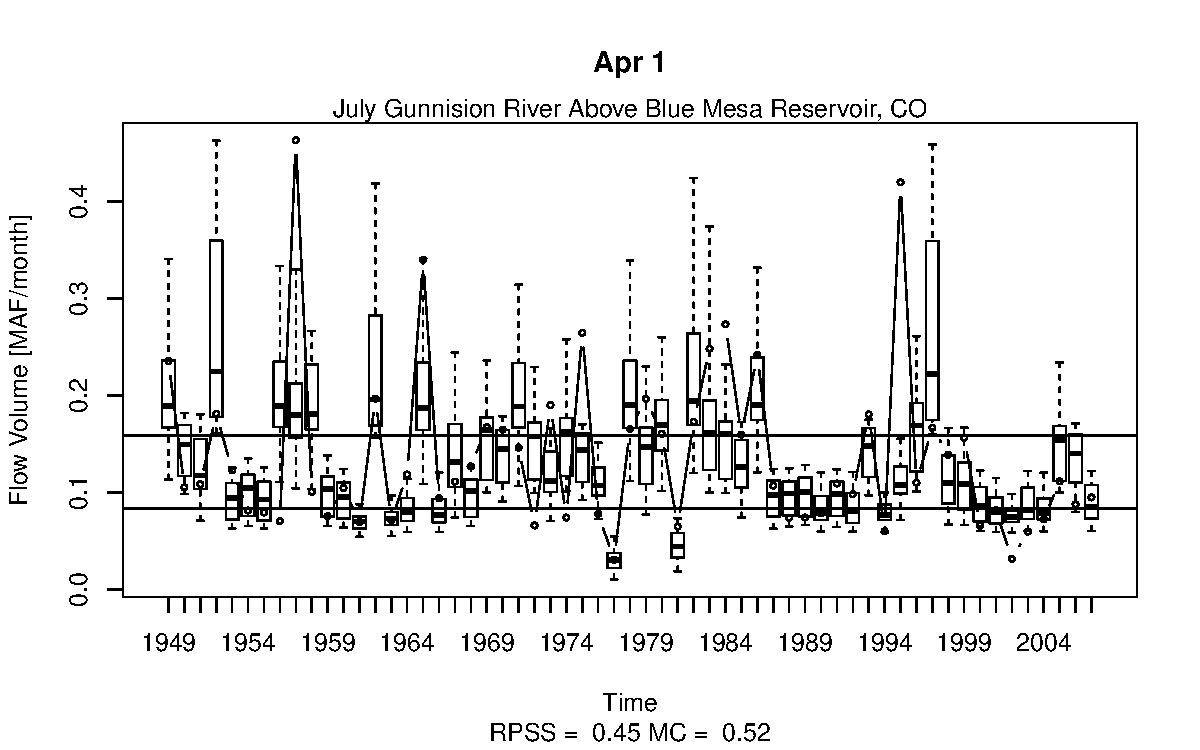
\includegraphics[width=\textwidth]{figs/Apr1_July_Gunnision_River_Above_Blue_Mesa_Reservoir,_CO_all_box.pdf}
\end{frame}

\section{Future Work}

\begin{frame}{Second Year Forecasts}

\begin{itemize}
\item In the second year snowpack and climate info is not available
\begin{itemize}
\item Incorporate paleo data
\end{itemize}
\item Conditional resampling of analog paleo years (Markov Chain)
\item Climate indices 
\item Time series dynamics
\begin{itemize}
\item Data suggests embedding dimension of 3
\end{itemize}
\item Merge with interdecadal methods
\end{itemize}

\end{frame}
\begin{frame}
\frametitle{Preliminary Results}
\includegraphics[width=.9\textwidth]{figs/fig-11yrm-q4.pdf}
\end{frame}


\section{~}

\end{document}  